\chapter{Numerical Methods}
\label{sec:methods}

\cleanchapterquote{FFT is the most important numerical algorithm of our lifetime.}{Gilbert Strang}{(1934)}

Section Introduction

\section{Monte Carlo Method }
\label{sec:methods:MC}
In this section we will briefly recall the principle of the Monte Carlo simulations and present algorithms to simulate the different processes that we have studied in the last chapter. The idea in the Monte Carlo method is to simulate $M$ sample paths of the stock price process $\mathbf{S}_m, m=1,\ldots,M$, under the corresponding model and for each path, compute the present value $P(\mathbf{S}_i)$ of the financial product. Then, by the law of the large numbers, we obtain the following proxy:
$$\hat{P}(\mathbf{S})=\frac{1}{M}\sum_{m=1}^M P(\mathbf{S}_m)\xrightarrow{M\to\infty} P(\mathbf{S}),$$
where $\mathbf{S}=(S(t_1),\ldots,S(t_N))$ is the realization of the stock price. The standard error of the estimate is given by
$$\text{SE} = \sqrt{\frac{1}{M-1}\sum_{i=1}^M \left(\hat{P}(\mathbf{S})-P(\mathbf{S}_i)\right)^2}.$$
Remark that the standard error decreases with the square root of the number of sample paths $M$.

Recall that in our case, the present value of the FX TARN is given by equation \eqref{eq:intro:pv}:
$$P(\mathbf{S}) =N_f \times \sum_{n=1}^N\frac{C_n(S(t_n),A(t_{n-1}))+C^\ast_n(S(t_n))}{B_d(t_0,t_n)}, \qquad A(t_0)=0,$$
where $C_n$ and $C_n^\ast$ are respectively the gain and the loss on the $n^\text{th}$ fixing date given by equations \eqref{eq:TARN:gain} and \eqref{eq:TARN:loss}. The variable $A(t_n)$ models the accumulated gains until the date $t_n$ and $B_d(t_0,t_n)^{-1}=e^{-r_d(t_n-t_0)}$ is the domestic discounting factor from $t_n$ to $t_0$. In the rest of the thesis, we will consider the present value per unit of notional $(N_f=1)$.

\subsection{Simulations under Black-Scholes model}
We have seen that the L\'evy process in the Black-Scholes model is given by
$$X_t^\text{BS} = \left(r-q-\frac{1}{2}\right)t +\sigma W_t,$$
where $W_t$ is a Wiener process. Therefore, by discretization of time, we get
$$\Delta X_t^\text{BS}=\left(r-q-\frac{1}{2}\sigma^2\right)\Delta t+\sigma \sqrt{\Delta t}Z,$$
with $Z\sim\mathcal{N}(0,1)$. Finally we easily have
\begin{align*}
S_{t+\Delta_t} &= \exp\left\{X_t^\text{BS}+\left(r-q-\frac{1}{2}\sigma^2\right)\Delta t+\sigma\sqrt{\Delta t}Z\right\}\\
&= S_t\exp\left\{\left(r-q-\frac{1}{2}\sigma^2\right)\Delta t+\sigma\sqrt{\Delta t}Z\right\}.
\end{align*}
We can use the command \textbf{\texttt{random('norm',0,1)}} in \textsc{Matlab} to generate random normal variable.
\begin{figure}[!htb]
	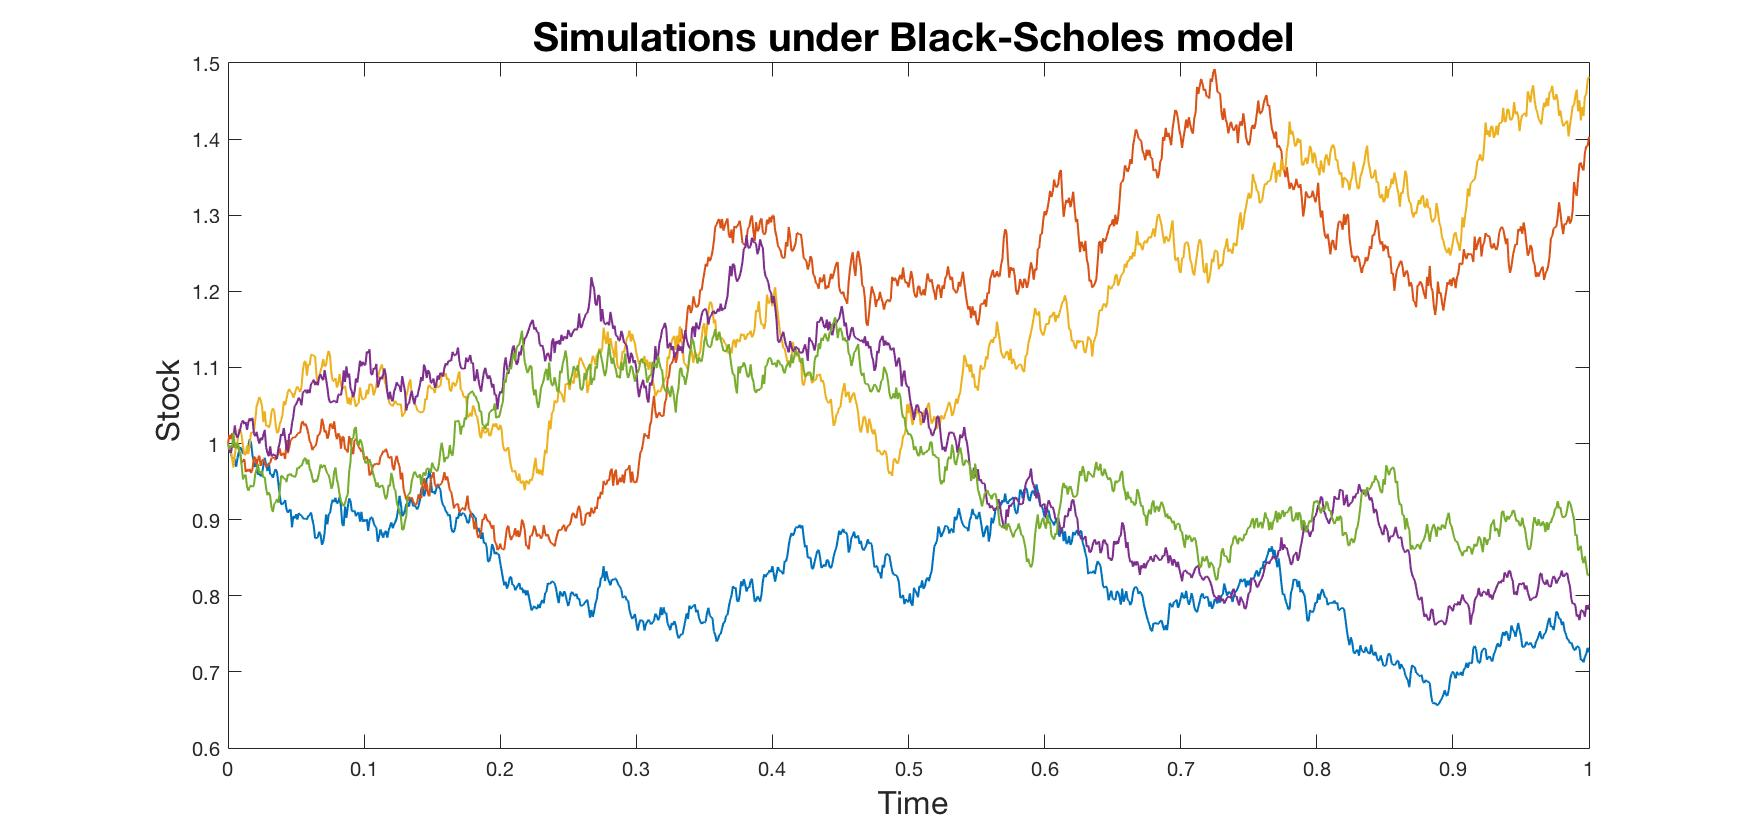
\includegraphics[width=\textwidth]{gfx/BS_plot}
	\caption{Simulations of stock price process under Black-Scholes model.\\ $S_0=1, r= 0.01,q = 0.02, \sigma=0.3, T = 1, dt = 0.001, M=5$.}
	\label{fig:MC:BS}
\end{figure}

\subsection{Simulations under Jump-diffusion models}
A jump-diffusion process is nothing else than a Brownian motion with drift to which is added by a jump process modeled by a compound Poisson process. In other words, we have
$$X_t^\text{JD} = \gamma^\ast t + \sigma W_t + \sum_{i=1}^{N_t}Y_i,$$
where $N_t\sim\text{Poisson}(\lambda t)$ and the jump size $Y_i$ has density function $f_J$. We have seen the two special case where the distribution $f_J$ is normal $\mathcal{N}(\alpha,\delta^2)$ in the Merton model and double exponential $\text{DoubleExp}(p,\eta_1,\eta_2)$ in the Kou model.

Therefore, we have that
$$\Delta X_t^\text{JD} = \gamma^\ast \Delta t + \sigma \sqrt{\Delta t} Z + J(\Delta t),$$
where $J(\Delta t)$ is the sum of all jumps between $t$ and $t+\Delta t$, i.e.
$$J(\Delta t)=\sum_{i=1}^{N_{\Delta t}}Y_i.$$
We can use the command \textsc{Matlab} \texttt{random('poiss',$\lambda \Delta t$)} to simulate the variable $N_{\Delta t}$.
\subsubsection{Merton model}
In his model, \citeauthor{Mer76} supposed that the jump size is normally distributed with mean $\alpha$ and standard deviation $\delta$, i.e. $Y_i\sim\mathcal{N}(\alpha,\delta)$. Then, recall that the risk-neutral drift is given by
$$\gamma^\ast = r-q-\frac{1}{2}\sigma^2-\lambda\left(e^{\alpha+\frac{1}{2}\delta^2}-1\right).$$
Thus we have
$$S_{t+\Delta t} = S_t\exp\left\{\gamma^\ast \Delta t + \sigma \sqrt{\Delta t}Z + J(\Delta t)\right\},$$
where $J(\Delta t)\sim\mathcal{N}(N_{\Delta_t}\alpha,N_{\Delta t}\delta)$ and $N_{\Delta t}\sim\text{Poisson}(\lambda\Delta t)$.

Finally, we obtain the results of five simulated sample paths in figure \ref{fig:MC:Mer}.
\begin{figure}[!htb]
	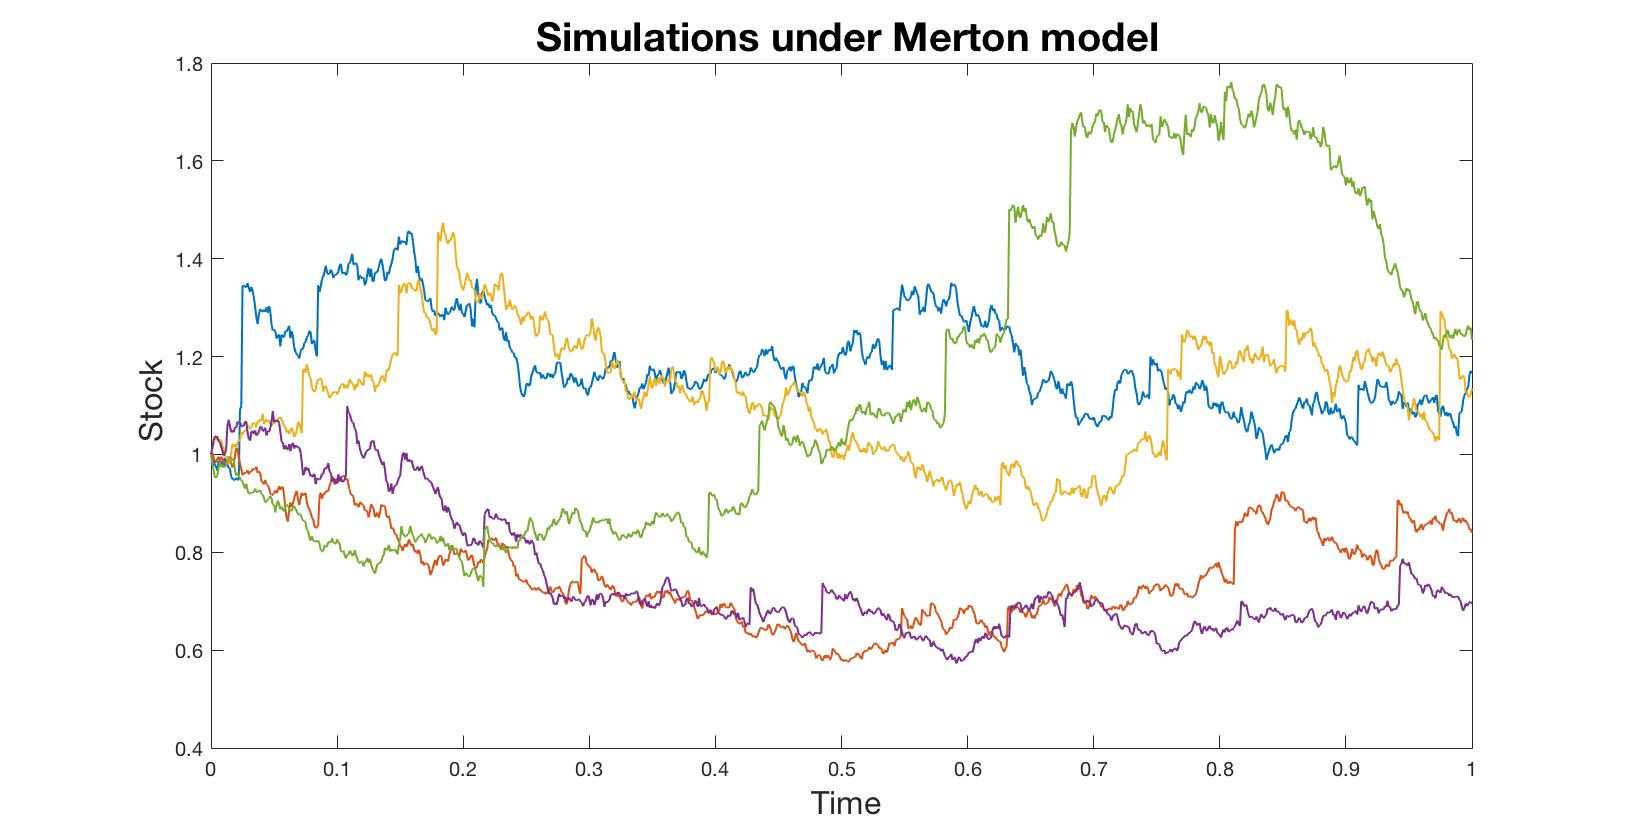
\includegraphics[width=\textwidth]{gfx/Merton_plot}
	\caption{Simulations of stock price process under Merton model.\\ $S_0=1, r= 0.01,q = 0.02,\lambda = 10 , \alpha = -0.05, \delta = 0.2, \sigma=0.3,$\\$T = 1, dt = 0.001, M=5$.}
	\label{fig:MC:Mer}
\end{figure}

\newpage
\subsubsection{Kou model}
This model is very similar to the Merton's one, but \citeauthor{Kou02} proposed to use a double exponential distribution for the jump size, i.e. $Y_i\sim\text{DoubleExp}(p,\eta_1,\eta_2)$. Thus the difficulty is to simulate double exponential random variables. Note that the sum of $K$ independent exponential random variables of parameter $\eta$ has a gamma distribution with parameters $K$ and $\eta$. In other words, if $X_1,\ldots,X_K\sim\text{Exp}(\eta)$, then $Y = \sum_{i=1}^K X_i\sim\Gamma(K,\eta)$ and
$$f_Y(y) = y^{K-1}\frac{\eta^K e^{-\eta y}}{K-1}.$$
Hence, to simulate the jumps $J(\Delta t)$, we begin by simulating a binomial random variable $K$ that counts the number of positive jump in $[t,t+\Delta t]$,
$$K \sim \text{Binomial}(N_{\Delta t},p), \qquad \text{ with } N_{\Delta t}\sim \text{Poisson}(\lambda\Delta t).$$
Then, we simulate the positive and negative jumps
\begin{align*}
J^+&\sim\text{Gamma}(K,\eta_1), \\
J^-&\sim\text{Gamma}(N_{\Delta t},\eta_2).
\end{align*}
Be careful using the \textsc{Matlab} command \texttt{random('gam',$K,1/\eta_i$)} because the convention of the parameters (shape/scale versus shape/rate).

Therefore the sum of jumps in the time interval $[t,t+\Delta t]$ is given by
$$J(\Delta t) = J^+-J^-.$$
At the end, we have the same representation of the stock price as before
$$S_{t+\Delta t} = S_t\exp\left\{\gamma^\ast \Delta t + \sigma \sqrt{\Delta t}Z + J(\Delta t)\right\},$$
with
$$ \gamma^\ast=r-q- \frac{1}{2}\sigma^2 -\lambda \left(\frac{p\cdot\eta_1}{\eta_1+1}+\frac{(1-p)\cdot\eta_2}{\eta_2+1}-1\right).$$
The simulation of sample paths under Kou model are illustrated in figure \ref{fig:MC:Kou}
\begin{figure}[!htb]
	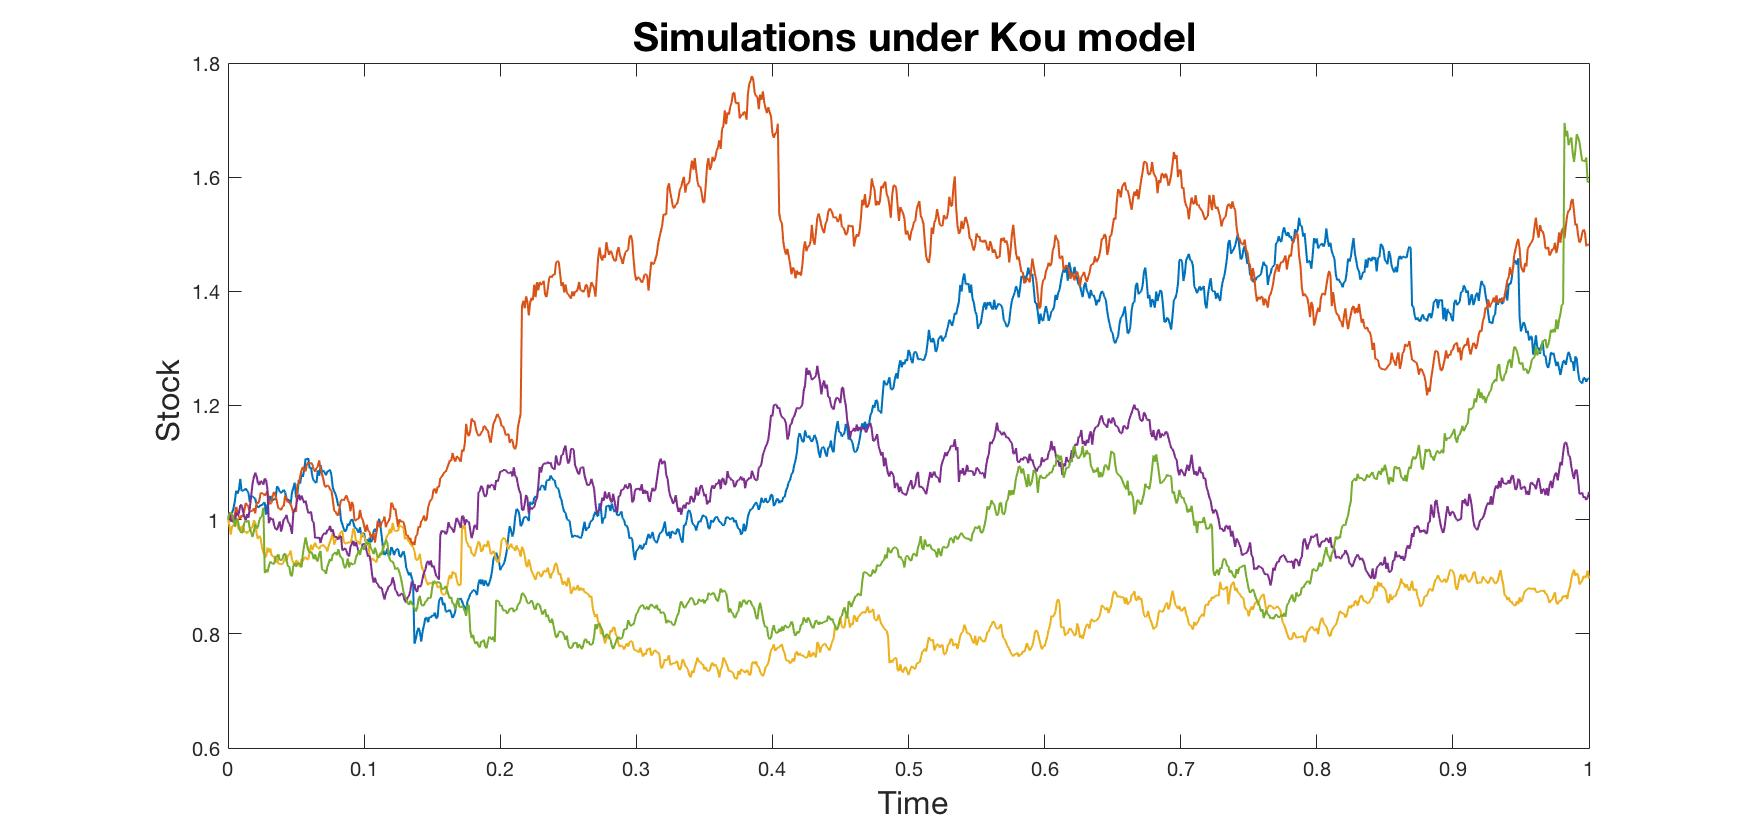
\includegraphics[width=\textwidth]{gfx/Kou_plot}
	\caption{Simulations of stock price process under Kou model.\\ $S_0=1, r= 0.01,q = 0.02,\lambda = 10 , p = 0.55, \eta_1 =\eta_2= 25, \sigma=0.3,$\\$T = 1, dt = 0.001, M=5$.}
	\label{fig:MC:Kou}
\end{figure}

\subsection{Simulations under Pure jump models}
Recall that a pure jump process can be seen as a Brownian subordination
$$X_t^\text{PJ} = \theta T_t + \sigma W_{T_t},$$
where $T=\left\{T_t,t\geq0\right\}$ is a random time process, called the \textit{subordinator}. The goal is then to simulate this subordinator and substitute it to the time into the Brownian motion with drift. In the Normal Inverse Gaussian model, this time subordinator will be a Inverse Gaussian process, and in the Variance Gamma model, it will be a Gamma process.

\subsubsection{Normal Inverse Gaussian model}
First of all, recall that the L\'evy process in the Normal Inverse Gaussian model is given by
$$X_t^\text{PJ} = \beta \delta^2 T_t + \delta W_{T_t},$$
with $T_t\sim \text{IG}\left(t,\delta \sqrt{\alpha^2-\beta^2}\right)$.
Hence we have to construct a Normal Inverse Gaussian (NIG) process. To do that, we simulate an Inverse Gaussian (IG) process and set it as time parameter of the Brownian motion. In fact, we have that
$$\Delta X_t^\text{PJ} = \beta\delta^2\Delta T_t+\delta \sqrt{\Delta T_t}Z, $$
where $\Delta T_t\sim\text{IG}\left(\Delta t, \delta \sqrt{\alpha^2-\beta^2}\right)$ and $Z\sim\mathcal{N}(0,1)$.

Finally, we have the stock price sample path
$$S_{t+\Delta t}=S_t\exp\left\{\gamma^\ast\Delta t + \Delta X_t^\text{PJ}\right\},$$
with $\gamma^\ast=r-q -\delta \left(\sqrt{\alpha^2-\beta^2}-\sqrt{\alpha^2-(\beta+1)^2}\right)$.
Be careful with the convention of the \textsc{Matlab} command \texttt{random('inversegaussian',$\mu,\lambda$)}, where $\mu = \frac{a}{b}$ is the mean and $\lambda = a^2$ is the shape parameter. We can see the result of five sample path in figure \ref{fig:MC:NIG}.
\begin{figure}[!htb]
	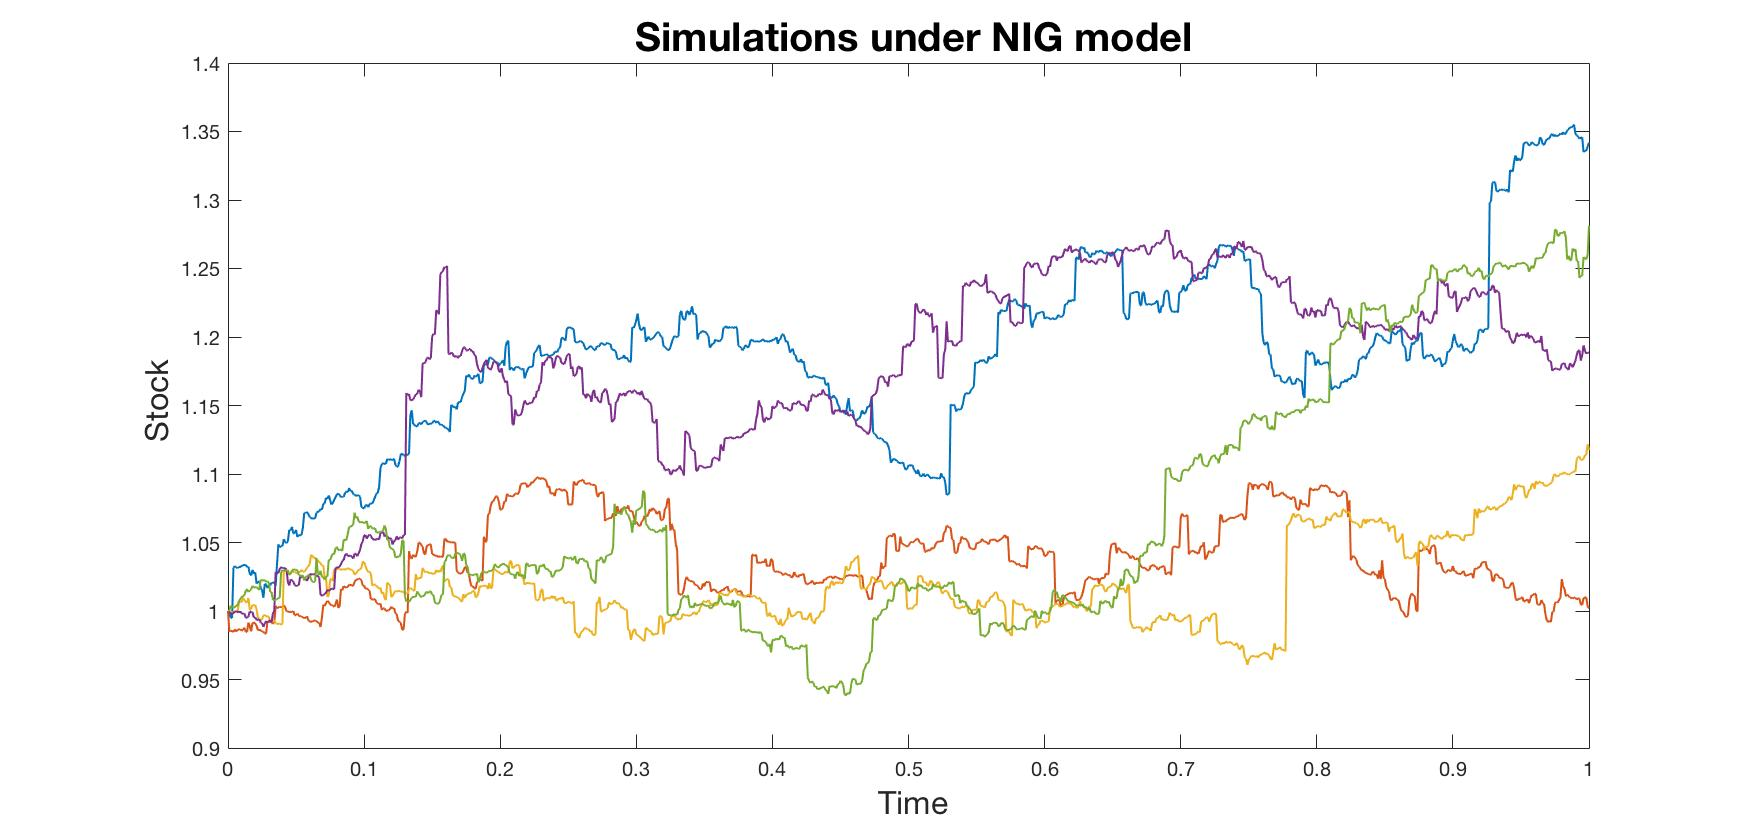
\includegraphics[width=\textwidth]{gfx/NIG_plot}
	\caption{Simulations of stock price process under NIG model.\\ $S_0=1, r= 0.01,q = 0.02,\alpha = 50 , \beta = 3, \delta = 1,$\\$T = 1, dt = 0.001, M=5$.}
	\label{fig:MC:NIG}
\end{figure}
\subsubsection{Variance Gamma model}
Following the same procedure as before, we just have to change the time subordinator process by taking a Gamma process. Then we have the time-changed Brownian motion
$$X_t^\text{PJ}=\theta T_t + \sigma W_{T_t},$$
with $T_t\sim \text{Gamma}\left(\frac{t}{\nu},\frac{1}{\nu} \right)$. Therefore, we get
$$\Delta X_t^\text{PJ} = \theta \Delta T_t + \sigma \sqrt{\Delta T_t} Z,$$
where $\Delta T_t\sim\text{Gamma}\left(\frac{\Delta t}{\nu},\frac{1}{\nu}\right)$ and $Z\sim\mathcal{N}(0,1)$.
Thus we get
$$S_{t+\Delta t} = S_t \exp\left\{\gamma^\ast\Delta t + \Delta X_t^\text{PJ}\right\},$$
with $\gamma^\ast = r-q + \frac{1}{\nu}\ln\left(1-\theta\nu-\frac{\sigma^2\nu}{2}\right)$.
The figure \ref{fig:MC:VG} illustrates the result of five simulations under this last model.
\begin{figure}[!htb]
	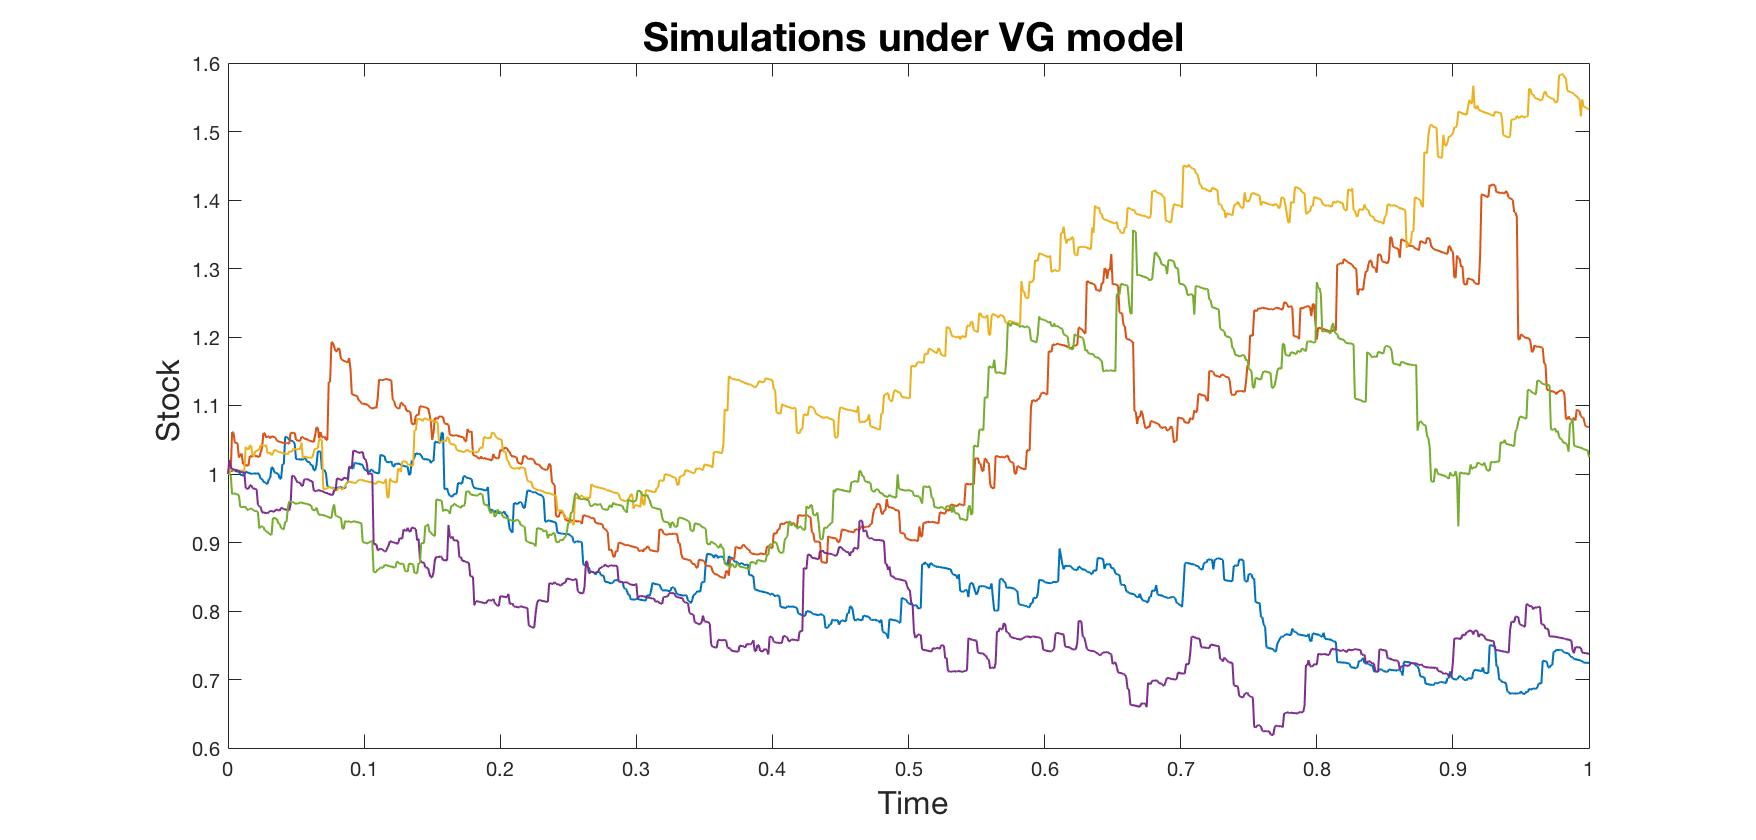
\includegraphics[width=\textwidth]{gfx/VG_plot}
	\caption{Simulations of stock price process under VG model.\\ $S_0=1, r= 0.01,q = 0.02,\theta = 0.5 , \sigma = 0.3, \nu = 0.01,$\\$T = 1, dt = 0.001, M=5$.}
	\label{fig:MC:VG}
\end{figure}
\subsection{FX TARN with Monte Carlo}
Note that for the pricing of the FX TARN it suffices to take $\Delta t$ equal to the difference of two consecutive fixing dates, i.e. the length of a period (e.g. Daily/Weekly/Monthly). This is not necessary to simulate the points between these dates because the cash flows depend only on the observations on the fixing dates.

From the simulations above, and equations \eqref{eq:TARN:gain} and \eqref{eq:TARN:loss}, this is easy to compute the payoff on each fixing dates $t_n, (n=1,\ldots,N)$, with respect to the realization $S_{t_n}$. This is also necessary to update the variable $A(t_n)$ that take into account the accumulated gain. 

Finally, we have for each simulated scenario $\mathbf{S}_m, (m=1,\ldots,M)$, the present value from equation \eqref{eq:intro:pv}
$$P(\mathbf{S}_m) = \sum_{n=1}^{N}e^{-r_d t_n}\left(C_n(S(t_n),A(t_{n-1}))+C^\ast_n(S(t_n))\right),$$
where we have taken $B_d(t_0,t_n)^{-1}=e^{-r_d (t_n-t_0)}$, with $r_d$ is the domestic risk-free rate. Hence, the value of the FX TARN obtained with Monte-Carlo method is given by
$$\hat{P}(\mathbf{S})=\frac{1}{M}\sum_{m=1}^M P(\mathbf{S}_m).$$

\section{Finite Difference Method}
\label{sec:methods:FD}

% \subsection*{Taylor Expansion}
% %Taylor Expansion
% Recall that the Taylor expansion for a function $f\in C^\infty$ infinitely many differentiable is given by
% \begin{align*}
% f(x) &= f(a) + (x-a)\frac{\partial f}{\partial x}(a) + \frac{(x-a)^2}{2!}\frac{\partial^2 f}{\partial x^2}(a) + \cdots + \frac{(x-a)^n}{n!}\frac{\partial^n f}{\partial x^n}(a)+\cdots\\
% &=\sum_{k = 0}^\infty \frac{(x-a)^k}{k!}\frac{\partial^k f}{\partial x^k}(a).
% \end{align*}

% If $f$ is only $(n+1)$ times continuously differentiable, i.e. $f\in C^{(n+1)}$, we can write
% $$f(x)=\sum_{k = 0}^{n+1} \frac{(x-a)^k}{k!}\frac{\partial^k f}{\partial x^k}(x)+O((x-a)^{n+1}),$$
% where $O((x-a)^{n+1})$ represents the remainder in Landau notation.

% \subsection*{Forward and Backward Difference Approximation of First Derivative}
% %Forward and Backward Difference Approximation of First Derivative
% In order to approximate $\frac{\partial f}{\partial t}(x)$ assume that $f$ is twice continuously differentiable, i.e. $f\in C^2$.  By a first order Taylor expansion we can write
% \begin{equation}\label{forwardTaylor}
% f(x + h) =  f(x) + h \frac{\partial f}{\partial x}(x)+ O(h),
% \end{equation}
% \begin{equation}\label{backwardTaylor}
% f(x - h) =  f(x) -h \frac{\partial f}{\partial x}(x)+ O(h).
% \end{equation}

% The equation \eqref{forwardTaylor} gives us
% \begin{equation}\label{fwd}
% \frac{\partial f}{\partial x}(x) =  \frac{f(x+h)-f(x)}{h} + O(h),
% \end{equation}
% which is known as \textit{forward difference} approximation of the first derivative. 

% On the other hand, the equation \eqref{backwardTaylor} gives us
% \begin{equation}\label{bwd}
% \frac{\partial f}{\partial x}(x) =  \frac{f(x)-f(x-h)}{h} + O(h),
% \end{equation}
% which is known as \textit{backward difference} approximation of the first derivative.

% \subsection*{Central Difference Approximation of First Derivative}
% %Central Difference Approximation of First Derivative
% Now assume that $f\in C^3$. Then with a second order Taylor expansion, we have
% \begin{equation}\label{forwardTaylor2}
% f(x+h) = f(x) + h \frac{\partial f}{\partial x}(x) + \frac{h^2}{2}\frac{\partial^2 f}{\partial x^2}(x) +O(h^2),
% \end{equation}
% \begin{equation}\label{backwardTaylor2}
% f(x-h) = f(x) - h \frac{\partial f}{\partial x}(x) + \frac{h^2}{2}\frac{\partial^2 f}{\partial x^2}(x) +O(h^2).
% \end{equation}

% Subtracting equation \eqref{backwardTaylor2} from  \eqref{forwardTaylor2} we get
% $$ f(x+h)-f(x-h) = 2h \frac{\partial f}{\partial x}(x) + O(h^2).$$

% Therefore we obtain the \textit{central difference} approximation of the first derivative
% \begin{equation}\label{cf1}
% \frac{\partial f}{\partial x}(x) = \frac{f(x+h)-f(x-h)}{2h} + O(h^2).
% \end{equation}

% \subsection*{Central Difference Approximation of Second Derivative}
% %Central Difference Approximation of Second Derivative
% Finally summing equations \eqref{forwardTaylor2} and \eqref{backwardTaylor2} we get
% $$2f(x) = f(x+h)+f(x-h)+ h^2 \frac{\partial^2 f}{\partial x^2}(x) + O(h^2).$$ 

% Then the \textit{central difference} approximation of the second derivative is given by
% \begin{equation}\label{cf2}
% \frac{\partial^2 f}{\partial x^2}(x) = \frac{f(x+h)-2f(x)+f(x-h)}{h^2}+O(h^2).
% \end{equation}

% \subsection*{Option Pricing under the Generalized Black-Scholes model}
% \label{sec:FD:GBS_PDE}
% %Option Pricing under the Generalized Black-Scholes model
% Consider the Generalized Black-Scholes model, which includes the \textit{local volatility} $\sigma(S,t)$ and term structures of \textit{interest rate} $r(t)$ and \textit{dividend rate} $q(t)$. The price of an asset $S$ under such model follows the \textit{stochastic differential equation} (SDE):
% $$dS_t = (r(t)-q(t))S_t dt + \sigma(S_t,t)S_tdW_t.$$

% Then we know that the value of an option $v(S,t)$ on that asset $S$ satisfies the following \textit{partial differential equation} (PDE):
% $$\begin{cases}
% \frac{\partial v}{\partial t} + \frac{\sigma(S,t)S^2}{2}\frac{\partial^2 v}{\partial S^2}+(r(t)-q(t))S\frac{\partial v}{\partial S}= r(t)v(S,t)\\
% v(S,T) = \Psi(S) & \text{Terminal Condition (Payoff function)}\\
% \frac{\partial^2 v}{\partial S^2}(S_{\max},t)=\frac{\partial^2 v}{\partial S^2}(S_{\min},t)=0 &\text{Neumann Boundary Conditions}
% \end{cases}$$

% Now if we use the change of variable $\tau = (T-t)$ to express \textit{time to maturity}, we obtain the following PDE:
% $$\begin{cases}
% -\frac{\partial v}{\partial \tau} + \frac{\sigma(S,\tau)S^2}{2}\frac{\partial^2 v}{\partial S^2}+(r(\tau)-q(\tau))S\frac{\partial v}{\partial S}= r(\tau)v(S,\tau)\\
% v(S,0) = \Psi(S) & \text{Initial Condition (Payoff function)}\\
% \frac{\partial^2 v}{\partial S^2}(S_{\max},\tau)=\frac{\partial^2 v}{\partial S^2}(S_{\min},\tau)=0 &\text{Neumann Boundary Conditions}
% \end{cases}$$

% To begin, we have to define the domain of the problem $$D = \{S_{\min}\leq S\leq S_{\max} ; 0 \leq \tau \leq T\}$$
% and set it to a discrete grid
% $$\bar{D} = \begin{Bmatrix}
% S_j = S_{\min}+(j-1)h; & h=\frac{S_{\max}-S_{\min}}{N}; & j = 1,\ldots,N+1 \\ t_k = 0 + (k-1)\Delta t; & \Delta t = \frac{T}{M}; &k = 1,\ldots,M+1 &
% \end{Bmatrix},$$
% where $N$ is the number of subintervals in the $S$-direction and $M$ is the number of subintervals in the $\tau$-direction.

% \subsection*{Forward Euler Approximation}
% %Forward Euler Approximation
% The Forward Euler approximation constructs the \textit{explicit} discretization of the Generalized Black-Scholes PDE. In other words, we approximate the theta term $\frac{\partial v}{\partial t}(S,t)$ using a \textit{forward difference} approximation \eqref{fwd}:
% $$\frac{\partial v}{\partial t}(S,t) \approx \frac{v(S,t+\Delta t)-v(S,t)}{\Delta t}.$$
% The \textit{central difference} approximation of the first derivative \eqref{cf1} for the delta term $\frac{\partial v}{\partial S}(S,t)$ gives us
% $$\frac{\partial v}{\partial S}(S,t) \approx \frac{v(S+h,t)-v(S-h,t)}{2h}$$
% and the \textit{central difference} approximation of the second derivative \eqref{cf2} for the gamma term $\frac{\partial^2 v}{\partial S^2}(S,t)$ gives
% $$\frac{\partial^2 v}{\partial S^2}(S,t) \approx \frac{v(S+h,t)-2 v(S,t)+v(S-h,t)}{h^2}.$$

% \subsection*{Backward Euler Approximation}
% %Backward Euler Approximation

% \subsection*{$\theta$-Method and Crank-Nicolson Approximation}
% %Theta-Method and Crank-Nicolson Approximation

\section{The Convolution Method}
\label{sec:methods:conv}
